\section{Introduction}
% WHERE: application in HRI
Robots operating in unstructured environments must weigh a delicate balance between adaptability and motion consistency. They are tasked with efficiently completing their designated tasks while ensuring safety in the presence of potential collisions, especially in the context of physical human-robot collaboration \parencite{ajoudani2018progress}.

% Fast control -> closed form DS
Central to effective robot control is the computation of desired velocities that guide them towards their goals. In complex and dynamic environments, real-time velocity adjustments based on real-time sensory information are essential. Achieving this necessitates algorithms that are easily configurable and capable of rapid evaluation. As such, closed-form control laws eliminate the need for frequent replanning. Dynamical Systems (DS) have emerged as a valuable framework for representing such desired motion. Where the behavior of the DS is approximated through suitable controllers. DS can be designed using established control theory tools to provide stability and convergence guarantees for navigating dynamic environments.

% Compliance [Stay Reactive]
In stark contrast to human musculature's remarkable ability to quickly adapt to external forces, most robotic systems consist of rigid metallic or plastic materials. Consequently, when these robotic systems interact with their environment, it often leads to abrupt energy transfers, posing the risk of damage to the robot itself or its surroundings. However, the advent of modern robotic platforms equipped with force and torque sensing capabilities has opened new avenues for precise control over the forces exerted by the robot.
Nonetheless, this advancement gives rise to a complex control challenge characterized by multiple constraints. The robot must achieve its designated position and maintain a desired velocity while remaining compliant with interaction forces. The control problem of balancing position, velocity, and force constraints, is addressed by \textit{impedance controllers} \parencite{takegaki1981new, hogan1984impedance}.

% Ensure Obstacle Avoidance
Effective obstacle avoidance is fundamental to motion control, with reactive approaches capable of handling dynamic and intricate environments \parencite{huber2019avoidance}. However, integrating obstacle avoidance with compliance control requires careful design. The controller should remain compliant in free space while adhering to the desired motion. Furthermore, when encountering surfaces like fragile glass on a table, the controller must adopt stiffness to prevent a collision, yet it should be compliant when interacting with an operator (Fig.~\ref{fig:table_avoidance_with_obstacle}). Achieving this necessitates a variable impedance controller, capable of weighting different objectives, such as dynamic motion and external force compliance \parencite{kronander2015passive}.

\begin{figure}
\centerline{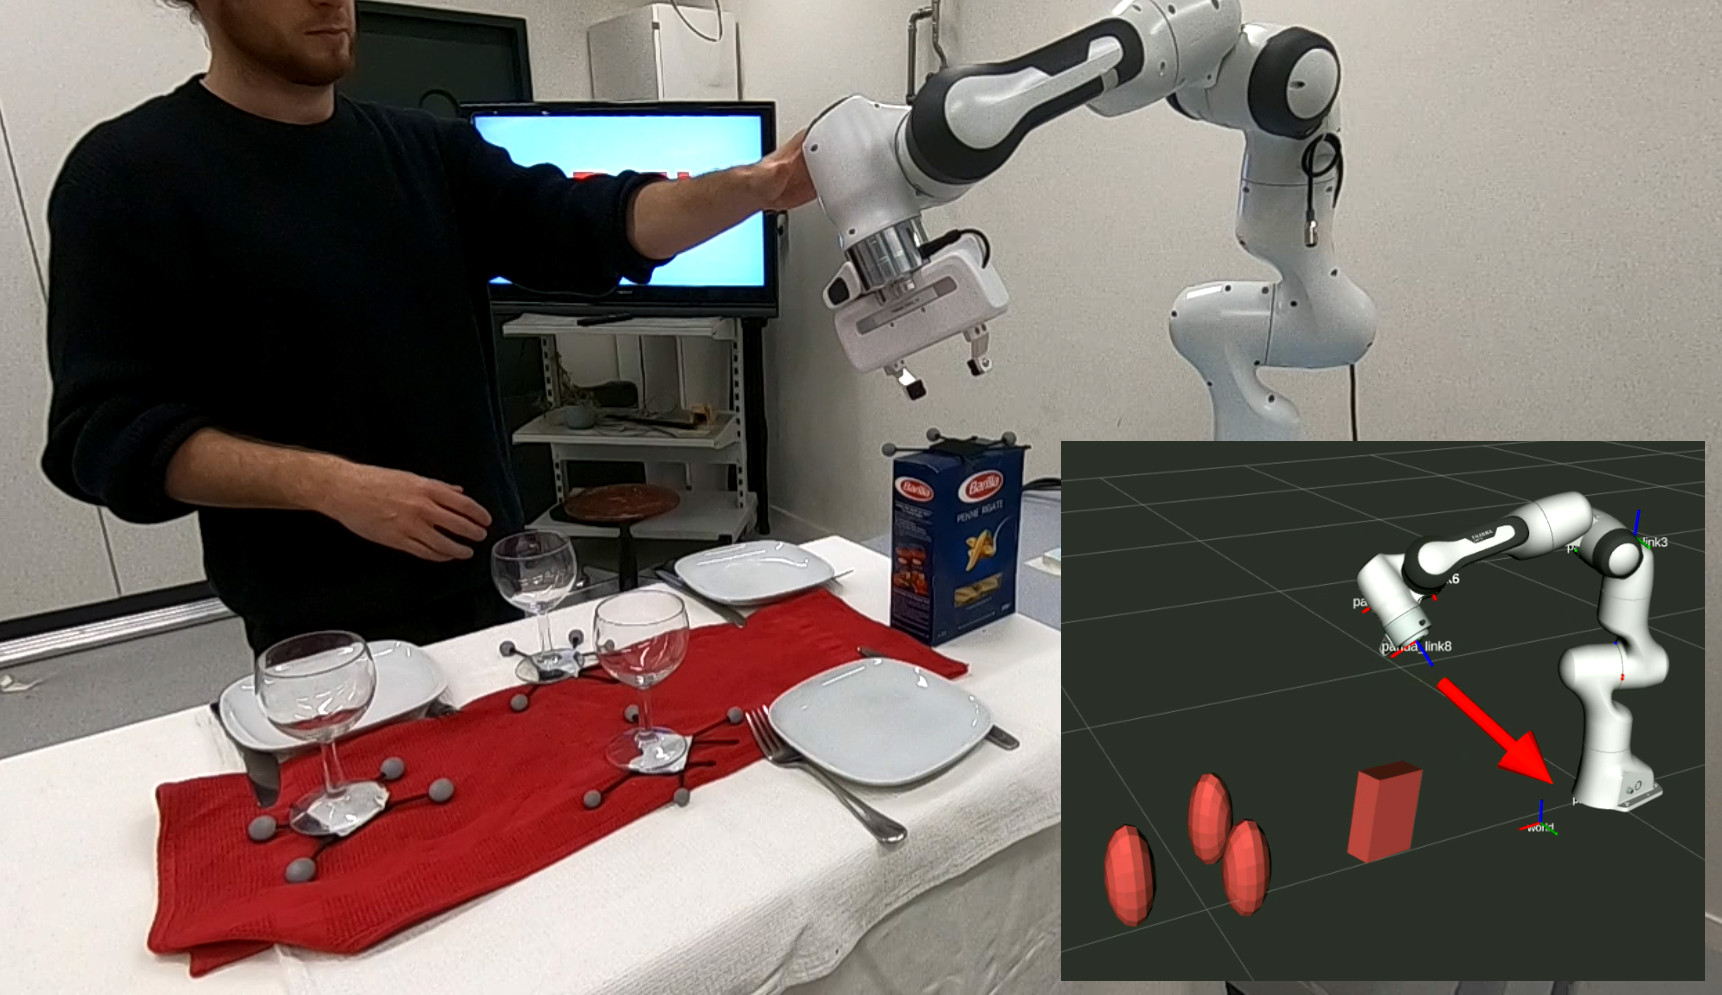
\includegraphics[width=1.0\columnwidth]{figures/robot_arm_table_avoidance}}
\caption{
The proposed passive obstacle-aware controller lets the robot absorb external disturbances while ensuring collision avoidance. 
While tipping over the closed pasta box on this dinner table setup might be acceptable. Yet, the delicate wine glasses demand careful handling to prevent breakage.
}
\label{fig:table_avoidance_with_obstacle}
\end{figure}

This work introduces a novel approach incorporating dynamic obstacle avoidance using DS and variable impedance control, enhancing adaptability, reactivity, and safety in robotic movements. It empowers robots to navigate complex environments proactively, avoiding collisions and rejecting disturbances. Our approach is evaluated through simulations and practical implementation on a 7-degree-of-freedom (7DoF) robot arm, demonstrating robust and safe control in real-world scenarios.

